\documentclass[10pt,a4paper,danish]{article}
\usepackage[danish]{babel}
\usepackage[utf8]{inputenc}
\usepackage{amsmath}
\usepackage{amssymb}
\usepackage{listings}
\usepackage{fancyhdr}
\usepackage{hyperref}
\usepackage{booktabs}
\usepackage{graphicx}
\usepackage{xfrac}
\usepackage[dot, autosize, outputdir="dotgraphs/"]{dot2texi}
\usepackage{tikz}
\usetikzlibrary{shapes}
\usepackage{multirow}
\usepackage{pdfpages}

\pagestyle{fancy}
\fancyhead{}
\fancyfoot{}
\rhead{\today}
\rfoot{\thepage}
\setlength\parskip{1em}
\setlength\parindent{1em}

%% Titel og forfatter
\title{Vurdering af projektstyringen i Tinglysningsprojektet}
\author{Maria Caroline Miller, 040779, twq135}

%% Start dokumentet
\begin{document}

%% Vis titel
\maketitle
\newpage

%% Vis indholdsfortegnelse
\tableofcontents
\newpage

\section{Indledning}
%Lidt om tinglysningsprojektet
Tinglysningsprojektet er et stort statsligt projekt, som er blevet igangsat for at gøre tinglysningen nemmere i fremtiden. Tinglysning er den offentlige registrering, efterprøvelse og offentliggørelse af rettigheder over fast ejendom, som huse, biler, løsøre, ægtepagter og andelsbeviser. Tinglysningsprojektet handler om at samle disse oplysninger i et elektronisk system, istedet for den gamle model, hvor det blev skrevet ned i bøger. 

Samtidig med at Domsstolsstyrelsen står for at gennemføre Tinglysningsprojektet, er man også igang domstolsreformen, der sørgede for oprettelsen af Tinglysningsretten i Hobro. Hermed vil tinglysningen blive flyttet fra de enkelte byretter, og fremefter ligge samlet i Hobro. 


\subsection{Virksomhedsbeskrivelse}
%Domstolsstyrelsen
%Tinglysning på den gamle facon
Domstolsstyrelsen, som er den direkte ejer af projektet, er en styrelse under Justitsministeriet. Det er Domstolsstyrelsen, der administrerer og udvikler de danske domstole. Styrelsen ledes af en bestyrelse og en daglig ledelse. Bestyrelsen består af en højesteretsdommer, to landsdommere, to byretsdommere, en repræsentation for det øvrige juridiske personale ved domstolene, to repræsentanter for det administrative personale ved domstolene, en advokat, og to medlemmer med særlig ledelsesmæssig og samfundsmæssig indsigt. Den daglige ledelse varetages af en direktør og en stab.

\subsection{Tinglysning før projektet}
Inden det nye it-system kom frem blev tinglysning foretaget i de forskellige byretter. Man havde i hver retskreds en bog med tinglysninger, som blev holdt ajour i hånden. Dette var selvfølgelig tidskrævende at alting skulle opdateres i hånden. Det var også besværligt når ting skulle slåes op, da man skulle finde den rette bog osv. Derfor besluttede man at lave dette projekt, for at få centraliseret tingene et sted, og gøre det nemmere at arbejde med.

\section{Problemformulering}
%Evt. er det endelige produkt blevet afleveret
%Taget fra opgaven
Problemformuleringen til denne opgave er:
\begin{itemize}
\item Diskutér i hvilket omfang Domstolsstyrelsen har opnået succes med projektet ud fra en vurdering af i hvilken grad forventede costs og benefits er realiseret.
\item Analysér hvilke forhold der har været afgørende for i hvilken grad costs og benefits er blevet realiseret hos Domstolsstyrelsen.
\item Vurdér hvilket risikoniveau projektet har kørt med, og vurder hvilke tiltag Domstolsstyrelsen kunne have gennemført med henblik på at mindske risikoniveauet.
\end{itemize}

\subsection{Afgrænsning}
%Faser fra Marchewka? Christian har brugt fase 1, 2 og 5.
%Måske bruge modenhedsanalysen?

%Følgende teoretiske materiale bruges: s. 50-53 + s. 212



\section{Teori og metode}
%Risikostyring, fordele (TBO - Total Benefit of Ownership), udgifter (TCO - Total Cost of Ownership) og værditilførelse (MOV - Measurable Organisation Value)

%Brug teori-billedet han altid viser i slides

%PLC og SDLC, s. 36, fig. 2.1

%Business case: figur 2.3, s. 43

Et IT-projekt har en livscyklus med forskellige faser, som man bør gennemgå når man skal gennemføre et IT-projekt. Denne kan ses på figur \ref{fig:SDLC} på side \pageref{fig:SDLC}. Denne indeholder forskellige faser, som alle er vigtige. Projekt planen gør at man kan styre projektet mens det forløber, og evalueringen gør at man lærer noget af den proces man har været igennem, sådan at det næste projekt kan blive endnu bedre.

\begin{figure}[h!]
    \centering
    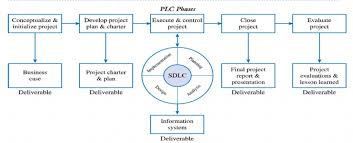
\includegraphics[width=0.8\textwidth]{SDLC.jpg}
    \caption{PLC - Product Life Cycle og SDLC - System Development Life Cycle \cite[~s. 36]{Marchewka}}
    \label{fig:SDLC}
\end{figure}

En af de vigtige ting at lave inden man starter er en business case. Det er her at man finder ud af om projektet overhovedet bør laves. Processen for udviklingen af en bussiness case kan ses i figur \ref{fig:business} på side \pageref{fig:business}. En business case består også af flere forskellige trin. Dem jeg vil koncentrere mig mest om i dette afsnit og opgave er trin 2, 5 og 6, som er den \textit{Measurable Organizational Value} (MOV), \textit{Total Cost of Ownership} (TCO) og \textit{Total Benefit og Ownership} (MBO). Derudover vil jeg også kigge på den del af trin 4, der drejer sig om risici. 

\begin{figure}[h!]
    \centering
    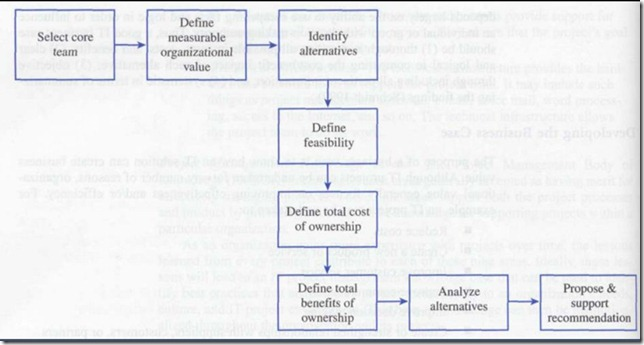
\includegraphics[width=0.8\textwidth]{business.jpg}
    \caption{Proces for udviklingen af en business case  \cite[~s. 43]{Marchewka}}
    \label{fig:business}
\end{figure}


\subsection{MOV, TBO- og TCO-modellerne}
%TBO og TCO: Marchewka s.52-53.
%MOV: Marchewka s. 44-50. fig 2.2 s. 50
%Marchewka s. 37
MOV drejer sig om at nedsætte nogle målbare kriterier for produktets succes. Kriterierne skal være målbare, da man på den måde med det samme kan se om man kan se nok fremgang ved at gå i gang med projektet. Det gør det også nemmere senere at evaluere på om projektet rent faktisk havde en indflydelse om man forventede. Et eksempel på et målbart kritere kunne være: Et år efter indførsel skal den enkelte ansatte kunne klare 25\% flere sager end i det gamle system. Dette indeholder både en effektivitetsmåling og en tidshorisont.

Et andet vigtigt punkt i business planen er at undersøge om omkostninger og fordele gør projektet interessant at arbejde videre med. Hvis omkostningerne er for store i forhold til de fordele der kommer ud af det, giver det ikke så meget mening at gennemføre projektet. TCO giver en oversigt over de omkostninger der er forbundet med projektet. Disse kan deles op i tre kategorier:

\begin{itemize}
\item Direkte: Køb af hardware og software, udvikling, konsulentlønninger etc.
\item Løbende: Lønninger, træning, opgraderinger, vedligeholdelse etc.
\item Inddirekte: Tab af produktivitet i begyndelsen, systemnedbrud, kvalitetssikring etc.
\end{itemize}

Som det kan ses på listen ovenfor \cite[~s. 53]{Marchewka} er der mange ting, som man skal beregne med i prisen for et projekt. Der er dog også for det meste fordele ved et projekt. Dette betegnes TBO. Disse involverer også både direkte, løbende og inddirekte fordele, og kan både være pengebesparelser på fx. lønninger (hvis man kan spare medarbejdere med det nye system), men kan også være fordelen at en sælger fx kan bruge mere tid på det reelle salgsarbejde og mindre tid på papirarbejde.


\subsection{Risikohåndtering}
%Risici bør have en så kontrolleret indvirkning som muligt. Negative risici bør kontrolleres, så de har en minimal påvirkning på resten af projektet.

%Marchewka (205-233):
%Risikocyklus

%Risk Management - Marchewka (205-239)

%s. 212, figur 8.2: Identificering af risici og opdeling

Når man starter et nyt projekt er det også vigtigt at kigge på de risici, der er forbundet med projektet. Dette er en vigtig del, fordi hvis noget går galt kan det ødelægge et helt projekt. En risikoanalyse bør fokusere på disse punkter \cite[~s. 52]{Marchewka}:

\begin{itemize}
\item Identifikation - Hvad kan gå galt? Er der noget der skal ske for at sikre success?
\item Vurdering - Hvad er påvirkningen af hver risiko?
\item Reaktion - Hvordan kan risikoen undgåes eller minimeres?
\end{itemize}

Hvis man tænker dette ind fra starten af, så har man allerede en løsningsmodel for de ting, som kan gå galt undervejs. Dette gør at det bliver nemmere at fortsætte projektet uden alt for store forsinkelser. Hvis nu fx. projektlederen undervejs bliver tilbudt et andet job, som personen ikke kan afslå, så risikerer man at skulle starte næsten forfra, da projektlederen sidder på enormt meget viden om projektet. Hvis nu man fra starten har indset at dette kunne være en mulighed, og derfor i kontrakten med projektlederen har indskrevet en længere opsigelsesperiode (så personen har god tid til at oplære en ny), eller en konkurrencedygtig løn og andre goder, kan man minimere risikoen for at projektet bliver forsinket pga dette.

Når man skal lave en risikostrategi er der typisk fire fremgangsmåder \cite[~s. 210]{Marchewka}:

\begin{itemize}
\item Accepter eller ignorer risikoen
\item Undgå risikoen helt
\item Formindsk sandsynligheden eller konsekvensen af risikoen (eller begge), hvis den opstår
\item Overfør risikoen til en anden (fx forsikring)
\end{itemize}

Det er vigtigt at man allerede inden man starter projektet har identificeret sine risici, og har givet den en af de fire løsningsmodeller ovenfor. Dette gør at man hurtigt kan gribe fat, og sørge for at der bliver taget de rette forholdsregler med det samme.



\section{Diskussion}
%Er succeskriterierne nået?
%MOV
%Målbare - slides 2, s. 8

%Opgaven om successkriterier

%Har offentlige projekter TCO og TBO?

I denne sektion skal vi kigge direkte på Tinglysningsprojektet. Vi skal have fundet svar på denne del af problemformuleringen: \textit{Diskutér i hvilket omfang Domstolsstyrelsen har opnået succes med projektet ud fra en vurdering af i hvilken grad forventede costs og benefits er realiseret.}

\subsection{MOV og succeskriterier}
Første del af diskussionen drejer sig om Tinglysningsprojektet har opnået deres succeskriterier. Det har været meget vanskeligt i det udleverede materiale at finde de succeskriterier, som projektet er blevet startet på baggrund af, men det er lykkedes mig at finde et par stykker. De nævnes på \cite[~s.33]{Rigs}. Succeskriterierne kan ses nedenfor:

\begin{itemize}
\item Tinglysningen af fast ejendom effektiviseres for alle aktører i sikkerhedsmæssigt trygge rammer
\item Man forbedrer kundeservicen væsentligt overfor borgeren ved at kunne præsentere valide tinglysningsdata i én samlet løsning, der kan foretages opslag i fra internettet.
\item Der opnås en række samfundsmæssige gevinster, idet borgerne fx kan spare udgifter til bl.a. kurssikring og mellemfinansiering
\item De professionelle aktører i form af banker, realkreditinstitutter, advokater og ejendomsmæglere via en særlig adgang til tinglysningssystemet, herunder eventuelt ved integration fra egne it-systemer, kan foretage anmeldelser og straks modtage svar fra Tinglysningsretten om resultatet af den automatiserede prøvelse "`på egen skærm"' 
\item Der vil ske en personalebesparelse på 200 årsværk
\end{itemize}

Umiddelbart er det jo tydeligt at disse succeskriterier ikke er specielt målbare, da de hverken indeholder en procentsats for tilfredshedsmåling, eller et tidspunkt hvor dette skal være indfriet. Det betyder dog ikke at man ikke kan kigge på om disse ting ikke godt kan være opfyldt tilfredsstillende alligevel.

Til baggrund for min diskussion vil jeg bruge Rigsrevisionens vurdering af de ovenstående kriterier \cite[~s. 34]{Rigs}, da vi ikke har Domstolsstyrelsens egen vurdering.

Besparelsen på personale er på sin vis opnået, da det at Tinglysningen blev samlet i Hobro har gjort at man har kunnet spare personale. Tidligere skulle der i hvert retskreds sidde folk til at håndtere tinglysningen tilfredsstillende, men nogle steder har de måske ikke haft lige så meget arbejde at udføre. Dette blev nu samlet i en mængde medarbejdere der passede svarende til mængden af sager fra hele landet. I starten var der selvfølgelig problemer fordi systemet var nyt, og der var ansat ekstra personale til at hjælpe i starten, men jeg synes det virker som om systemet fungerer nu. Der er dog blevet tilføjet ekstra ressourcer til Tinglysningsretten i 2009, hvilket gør at effektiviseringsgevinsten reelt nok er mindsket.

Punktet om at tinglysningen skal effektiviseres er delvist løst, da den digitalte tingbog er blevet idriftsat pr. september 2009, men at de tre andre bøger stadig mangler at blive idriftsat. Dermed mangler man stadig Andelsbogen, for at have tinglysning af fast ejendom på plads.

De professionelle aktører har fået deres effektivisering, da 70\% af alle anmeldelser nu klares automatisk "`egen skærm"' via internettet. Dette giver meget bedre arbejdsvilkår for denne gruppe. Samtidig er kundeservicen for borgere og virksomheder steget, da de nu nemt kan slå ting op omkring tinglysningen over internettet. Systemet har dog fået ry for ikke at være super brugervenligt, men man kan jo håbe at det er noget som der bliver arbejdet på i fremtiden.

\subsection{TCO og TBO}
I Rigsrevisionens rapport har vi et helt afsnit omkring økonomien og vi får forelagt det oprindelige budget for projektet \cite[~s. 36]{Rigs}. I dette budget kan det tydeligt ses at det forventes at projektet begynder at give overskud halvandet år efter igangsættelsen, som på dette tidspunkt har været sat til midten af 2008. Det er jo klart at da projektet bliver udskudt, stiger udgifterne til færdiggørelse, og besparelserne på personale træder ikke i kraft på samme tid. Det er dog tydeligt og også Rigsrevisionens vurdering at dette budget ikke indeholder alle de udgifter, som man må forvente ved et system, og heller ikke alle besparelserne. Det er derfor tydeligt at Domstolstyrelsen ikke har arbejdet grundlæggende godt nok med at udføre deres TCO, og de derfor mister noget overskuelighed over hvormeget værdi projektet har.

TBO er i Tinglysningsprojektet uløseligt forbundet med MOV og de succeskriterier, som der er opstillet. Det er dog svært at se hvilke fordele selve Domstolstyrelsen og Tinglysningsretten fået ud af projektet andet end en besparelse på 200 årsværk. De fleste fordele er for brugerne og de eksterne aktører. Da Tinglysningsprojektet er et offentligt projekt betalt af staten har vi ikke helt de samme behov for TBO, da denne er svær at måle for offentlige projekter. Ejeren af projektet har typisk ikke de store fordele ved projekterne, men de hjælper ofte den almene borger.

\section{Analyse}
%Hvilke forhold har været afgørende for realisering?

%Fase 5 side 39
Anden del af problemformuleringen handler om de faktorer der har været grundlaget for realiseringen af projektet: \textit{Analysér hvilke forhold der har været afgørende for i hvilken grad costs og benefits er blevet realiseret hos Domstolsstyrelsen}.

Der har været en del faktorer, som har haft indflydelse på projektet gennem forløbet. En af de faktorer som nok gav den største forsinkelse var at leverandøren CSC mistede en stor del af sine erfarne udviklere i løbet af projektet. De blev headhuntet til andre virksomheder, og leverandøren stod pludselig og manglede erfaren arbejdskraft. Dette gjorde at projektet blev udskudt i 7 måneder, mens CSC fik ansat nye medarbejdere og opkvalificeret de resterende medarbejdere. 
"`Konkurrenters headhunting af centrale ansatte hos it-firmaet CSC kommer næste år til at koste både boligejere, banker, realkreditinstitutter, advokater og ikke mindst statskassen op imod 300 mio. kr. i form af gevinster, der var blevet stillet i udsigt af Domstolsstyrelsen."'\cite{Epn}
 
En af de andre beslutninger, som viste sig at have katastrofale konsekvenser for almindelige borgere var beslutningen om at udføre projektet som et Big Bang projekt. Dette betyder at projektet blev rullet ud over hele landet samtidig, og det gamle system blev lukket fra samme dag. Da projektet allerede var blevet forsinket to gange, kunne regeringen og Domstolsstyrelsen ikke klare endnu en forsinkelse, og derfor blev systemet taget i brug i september 2009. Hvis man havde startet med at sætte systemet i drift i en enkelt retskreds, så ville man have opdaget problemerne uden at det fik alvorlige konsekvenser for folk i hele Danmark. Nu skete der det at mange folk måtte beholde deres dyre mellemfinansieringslån mens de ventede på sagsbehandlingen.

Grundet forsinkelserne var der heller ikke tid til at gennemteste systemet sådan som man havde ønsket. Finanssektoren fik ikke den tre måneder lange prøvetid, som de gerne ville have\cite{Inf}, og advokater og ejendomsmæglerne fik slet ikke lov til at teste systemet inden det blev sat i drift. Hvis man nu havde ladet projektet tage endnu en forsinkelse og dermed havde åbnet op for muligheden for at systemet kunne blive ordentligt testet af brugerne, så ville man nok have opdaget problemerne med fx digital signatur. Systemet var nemlig sat op til at brugerne selv kunne bruge deres digitale signatur, og derved nemt kunne oprette sig i systemet. Problemet var at de fleste folk ikke havde digital signatur, og derfor istedet udfyldte en fuldmagt, så deres ejendomsmægler/advokat kunne bruge deres signatur istedet. Dette gav en hel masse ekstraarbejde for Tinglysningsretten, som man altså ikke havde forudset. Denne ting kunne højest sandsynligt have været undgået hvis ejendomsmæglere osv havde fået lov at teste systemet inden.

I aflevering 5\ref{app:vandfald} lavede vi en gennemgang af metoder for projektet, og fandt frem til at den metode, der blev brugt er den såkaldte vandfaldsmetode. Som beskrevet i opgaven: "`Det at projektet at fastlagt fra starten af er dog også en af de store risci ved vandfaldsmetoden. Metoden gør at projektet ikke tager højde for at virkeligheden og behovene kan ændre sig undervejs i udviklingen. Dette gør at når projektet endelig er færdig, kan det være totalt utidssvarende, hvilket kan gøre at projektet aldrig bliver sat i drift, eller at der skal bruges en hel masse penge på at føre systemet up to date."' Dette har højest sandsynligt netop været problemet med den digitale signatur. Da projektet blev oprettet i sin tid var den digitale signatur stadig helt ny, og man har højest sandsynligt forventet at det ville sprede sig mere og mere gennem udviklingsperioden. Da dette ikke skete, og næsten ingen mennesker skaffede sig en digital signatur, var det dog allerede for sent at ændre noget ved, da dele af systemet var færdigt, og man skulle videre til de næste dele.




\section{Risikovurdering}
%Hvilket risikoniveau har projektet kørt med?
%Mediestrategi?

%Risk management processes s. 209, figur 8.1

%Risikoniveau: tabel med elementer fra 5 lags framework
%Typen: figur 8.4, s.212




\subsubsection{Risikoidentifikation}
Jeg har valgt at tage udgangspunkt i de risici, som vi selv i aflevering 3 fandt som værende de vigtigste risici. Disse er bestemt ud fra et bredt kendskab til selve Tinglysningsprojektet, og vi fandt dengang at de opsummerede meget godt de punkter, som Rigsrevisionen har med fra Domstolsstyrelsens egen risikoanalyse \cite[~s. 18]{Rigs}. Vi havde desværre ikke adgang til denne analyse.

Vi har identificeret følgende 6 risici:
\begin{itemize}
\item Idriftsættelsesstrategien giver bagslag
\item Effektiviteten ved systemets ibrugtagen er ikke som forventet
\item Ansatte flytter ikke med til Hobro 
\item Nøglepersoner forlader projektet
\item Leverandør udfører ikke arbejdet hurtigt nok
\item Kunde kommer med for mange ændringer
\end{itemize}


\subsubsection{Risikovurdering}
%Risikomatrice christians opgave s. 16
Vi har lavet en tabel der viser betydningen af de forskellige risici. X-aksen viser konsekvensen af de forskellige risici på en skala fra 1-5, og y-aksen viser sandsynligheden for at problemet opstår på en skala fra 1-5.

\begin{tabular}{l|l|l|l}
           & 0-100\%       & 0-10       & P*I   \\
Risiko     & Sandsynlighed & Konsekvens & Score \\\hline
Idriftsættelse & 70\% & 9 & 6,3 \\
Effektivitet   & 90\% & 4 & 3,6 \\
Flytning   & 90\% & 5 & 4,5 \\
Nøglepersoner & 40\% & 4 & 1,6 \\
Leverandør & 70\% & 6 & 4,2\\
Ændringsforslag & 70\% & 7 & 4,9 \\
\end{tabular}

Som man kan se af tabellen er der ekstremt stor sandsynlighed for at projektet løber ind i et eller flere af disse problemer. Næsten alle de risici, som vi har fundet har høj sandsynlighed, og flere af dem vil også have omfattende konsekvenser. Man må derfor indse at dette projekt er et højrisikoprojekt, og skal behandles som et sådant.

Et højrisikoprojekt betyder at projektet er meget udsat for påvirkninger, der kan skabe forsinkelser eller have en anden ødelæggende effekt på projektet. Når der er tale om et højrisikoprojekt er det derfor ekstremt vigtigt at man allerede tidligt i processen er opmærksom på de ting, som der kan gå galt, sådan at man kan nå at reagere på dem inden de udvikler sig alvorligt. Det er derfor enormt vigtigt at have en ordentlig risikostrategi.

Som man kan se på tabel 2 i \cite[~s. 20]{Rigs} mente Domstolsstyrelsen selv ved projektets start at der var tale om et mellemrisikoprojekt. Selvom de organisatoriske forhold scorer højt, har de slet ikke forudset at der kunne komme problemer hos leverandøren, og giver dem en lav risiko. Rigsrevisionen vurderer i deres tekst at Domstolsstyrelsens risikoanalyse og deres tabeltal ikke passer sammen, og at projektet til alle skulle have været vurderet som et højrisikoprojekt. Dette er især set ud fra at tidsplanen for projektet er meget stram, samtidig med at det er et meget komplekst stykke software, der skal udvikles baseret på en stort set uafprøvet teknologi.


\subsubsection{Risikostrategi}
%s. 210
Som nævnt i teoriafsnittet er det vigtigste ved identificering af risici næsten at man lægger en strategi for hvordan man skal reagere, skulle den nævnte risiko indtræffe. Jeg har ikke på nogen måde kunne se at Domstolsstyrelsen har fremlagt noget risikostrategi, og det har højest sandsynligt været et af problemerne. Erik Frøkjær nævner i sin artikel \cite{Erik} nogle strategier, som man burde have igangsat. Et af de store problemer med systemet ved opstart var manglen på kvalificeret arbejdskraft. Dette var noget som man udemærket var klar over, men som stadig 5 dage inden opstart stadig var åbent og usikkert belyst. Man vidste simpelthen ikke hvad man skulle gøre ved problemet. "`Havde DSS gennemført selv ret elementære forsøg med prototype-versioner af det nye system, med et fornuftigt udvalg af sager dækkende de væsentligste sagstyper, og med et mix af erfarne og nye medarbejdere i Tinglysningsretten i Hobro, så havde man stået med et ganske andet og mere realistisk skøn over personalebehovet."' 

Et andet problem som viste sig at være af stor betydning var problemet med papirpantebreve. Man var klar over at der kunne være en risiko for at brugerne af systemet ville indsende papirpantebreve til skanning, men man havde ikke sørget for at lægge en strategi for at undgå dette problem. Havde man nu i god tid sørget for at lave en bindende aftale med brugerne om ikke at indsende disse i opstarten, så havde man sluppet for den store arbejdsmængde af 200.000 papirpantebreve, der skulle skannes. 

Som tidligere nævnt kunne man også sagtens have forudset problemerne med den digitale signatur. I Centraladministrationen har man tydeligt overblik over hvor få danskere der på dette tidspunkt anvender digital signatur til i vigtige sager, og havde man været i tvivl ville en lille brugerundersøgelse sagtens have kunnet vise dette. Dette har man jo vist længe, og man ville derfor have kunnet sørge for at ens strategi for dette netop havde været at ansætte flere medarbejdere, da man højest sandsynligt ville få en masse papirfuldmagter, der skulle sørges for.


\subsubsection{Risikoevaluering}
%s. 210
Det er tydeligt gennem den foregående analyse af risici at vi har at gøre med et højrisikoprojekt. Dette har Domstolsstyrelsen også efterfølgende erkendt ifølge Rigsrevisions rapport \cite{Rigs}. Man kan se at 4 ud af de 6 risici direkte skete, og de andre to (flytning og ændringer) kan sagtens have givet problemer, men det har vi ikke haft materiale om, og har derfor ikke kunnet undersøge det.

Det er vigtigt at afslutte sit projekt med at evaluere på sine risici. Derved har man mulighed for at lære af sine fejl, og måske undgå at lave de samme fejl næste gang.


\section{Konklusion}
Der er mange ting, der gik galt undervejs med Tinglysningsprojektet, og en hel del af dem kunne helt sikkert have været undgået, hvis man havde lavet et bedre projektarbejde i starten. Hvis man fra starten af havde nedskrevet ordentlige succeskriterier, hvis man havde undersøgt risici, konsekvenser


\section{Litteraturliste}
\begin{thebibliography}{9}

\bibitem{Erik}
  Erik Frøkjær
  \emph{Om den digitale tinglysningsskandale}
  Bragt i Ingeniøren på Version 2
  3. september 2010

\bibitem{Epn}
  \emph{http://epn.dk/teknologi2/branchen/article1177779.ece}
  4. april 2014, kl. 19.30

bibitem{Inf}
  \emph{http://www.information.dk/229579}
  4. april 2014, kl. 20.00

\bibitem{Krav}
  Devoteam Consulting
  \emph{Bilag 2: Kravspecifikation for det kommende
  system til elektronisk tinglysning}
  26. juni 2006

\bibitem{Marchewka}
  Jack T. Marchewka,
  \emph{\LaTeX: Information Technology Project Management}.
  John Wiley \& Sons, Inc.
  3nd Edition,
  2010.

\bibitem{Rigs}
  Rigsrevisionen,
  \emph{Beretning til Statsrevisorerne om det digitale   
  tinglysningsprojekt}
  August, 2010

\bibitem{Tid}
  \emph{Bilag 1: Hovedtidsplan}
  26. juni 2006

\bibitem{Wiki}
  \emph{http://da.wikipedia.org/wiki/Domstolsstyrelsen}
  3. april 2014, kl. 22.50

\end{thebibliography}

\newpage
\appendix
\section{Aflevering 5}
   \label{app:vandfald}
\includepdf[pages={2-}]{../uge5/aflevering5.pdf}

\section{Aflevering 3}
\label{app:uge3}
\includepdf[pages={2-}]{../uge3/aflevering3-gen.pdf}



\end{document}
